\chapter{Grids with Side Length at Least Five}

Recall from Definition \ref{defn:thickness} that $G(a_1,a_2,a_3)$ represents the $[a_1] \times [a_2] \times [a_3]$ grid $G$, and that $\min\{a_1,a_2,a_3\}$ is the thickness of $G$. For example, the tuple $G(5,3,3)$ represents the thickness 3 grid $[5] \times [3] \times [3]$. In the following lemmas, we use the notation $(a_1,a_2,a_3)+(x_1,x_2,x_3) = (a_1+x_1, a_2+x_2, a_3+x_3)$ to represent an instance of Corollary \ref{cor:recursion} on the $3 \times 2$ matrix $A$:
$$A =
\begin{bmatrix}
a_1 & x_1 \\
a_2 & x_2 \\
a_3 & x_3
\end{bmatrix}.
$$
For example, the expression $(5,3,3) + (3,3,3)$ indicates an application of Corollary \ref{cor:recursion}, using the matrix $A = \begin{bsmallmatrix} 5&3&3 \\ 3&3&3 \end{bsmallmatrix}^T$, to obtain the tuple $(8,6,6)$. 

We shall call a thickness \emph{complete} if it can be shown that all divisibility cases in that thickness admit perfect lethal sets. In this section, we demonstrate that thickness 5, thickness 6 and thickness 7 are all complete. As these belong to the residue classes 2, 0, and 1 modulo 3, respectively, we then use Lemma \ref{lem:plus_333} to show that all larger grids are also complete. 

\section{Completeness of Thickness 5}
We show that all divisibility cases for grids of thickness 5 admit perfect lethal sets. Observe that divisibility cases for thickness 5 consist of grids $G(x,y,5)$ where $x$ and $y$ are in residue classes $\{0,2,3,5\}$ modulo 6 (see Table \ref{fig:thickness_5_cases}). We separate these divisibility cases into the following four cases and show that each case is complete:

\begin{enumerate}
\item $G(x,5,5)$ for $x \in \{2,5\} \pmod 6$ and $x \geq 5$;
\item $G(x,6,5)$ for $x \in \{0,3\} \pmod 6$ and $x \geq 5$;
\item $G(x,y,5)$ for $x,y \in \{0,2,3,5\} \pmod 6$, $x \not\equiv y \pmod 6$ and $x \geq 5$;
\item $G(x,y,5)$ for $x,y \in \{0,2,3,5\} \pmod 6$, $x \equiv y \pmod 6$ and $x \geq 5$;
\end{enumerate}

\begin{table}[]
\centering
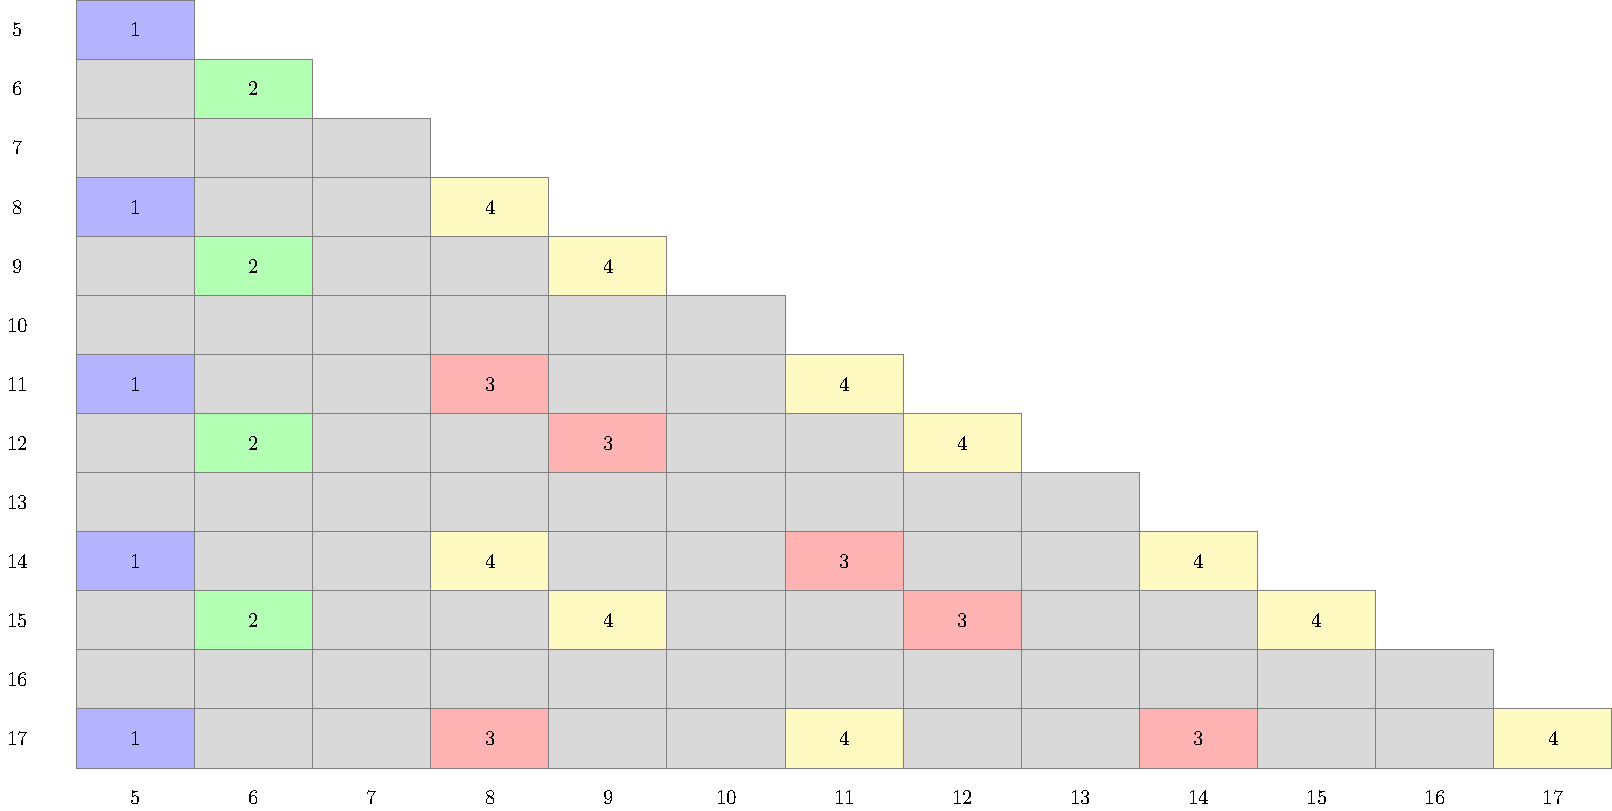
\includegraphics[width=\textwidth]{tables/4/thickness_5_cases.pdf}
\caption{The four thickness 6 cases analyzed in Lemmas \ref{lem:thickness_5_case_1} (blue), \ref{lem:thickness_5_case_2} (green), \ref{lem:thickness_5_case_3} (red), and \ref{lem:thickness_5_case_4} (yellow).}
\label{fig:thickness_5_cases}
\end{table}

%Leveraging \{lemmas from earlier chapters yet to be written\}, we show that all divisibility cases in thickness 5 percolate at the lower bound. 

%NOTE: THE FOLLOWING LEMMAS HOLD ASSUMING WE HAVE A GENERAL CONSTRUCTION FOR $(2,3,3k)$ FOR ALL $k$.
\begin{lem}
\label{lem:thickness_5_case_1}
All grids $G(x,5,5)$ for $x \in \{2,5\} \pmod 6$ and $x \geq 5$ admit perfect lethal sets.
\end{lem}

\begin{proof}
Consider $(5,2,2) + (a,3,3)$, for $a \equiv 0 \pmod 3$ and $a >3$. Observe that $(5+a,5,5)$ obtains all grids of the form described in Case 1, apart from $G(5,5,5)$ and $G(8,5,5)$.

By Corollary \ref{cor:recursion}, it suffices to show that $(5,2,2), (5,3,3), (a,2,3), (a,3,2)$ are all perfect. We have that $(5,2,2)$ is perfect by Construction \ref{con:5x2x2} in Appendix A, and $(5,3,3)$ is given by Proposition \ref{prop:3x3xk}. Since $a >3$, Propositions \ref{prop:2x3xk_0} and \ref{prop:2x3xk_3} give $(a,2,3)$. 

By Theorem \ref{thm:hypercubes} and Construction \ref{con:8x5x5} in Appendix A, we obtain the remaining grids $(5,5,5)$ and $(8,5,5)$, respectively. We conclude that all grids in Case 1 admit perfect lethal sets.
\end{proof}

\begin{lem}
\label{lem:thickness_5_case_2}
All grids $G(x,6,5)$ for $x \in \{0,3\} \pmod 6$ and $x \geq 5$ admit perfect lethal sets.
\end{lem}

\begin{proof}
Consider $(6,3,2) + (a,3,3)$, for $a \equiv 0 \pmod 3$ and $a >3$. Observe that $(6+a,6,5)$ obtains all grids of the form described in Case 2, apart from $G(6,6,5)$ and $G(9,6,5)$.

By Corollary \ref{cor:recursion}, we must show that $(6,3,2), (6,3,3), (a,3,3), (a,3,2)$ are all perfect. Since $a >3$, $(6,3,2)$ and $(a,3,2)$ are given by Propositions \ref{prop:2x3xk_0} and \ref{prop:2x3xk_3}. Similarly, $(6,3,3)$ and $(a,3,3)$ are given by Proposition \ref{prop:3x3xk}.

To obtain $(6,6,5)$, we consider $(3,3,1)+(3,3,4)$. By Corollary \ref{cor:recursion}, we must show that $(3,3,1), (3,3,4), (3,3,4), (3,3,1)$ are all perfect. These are obtained, respectively, by Propositions \ref{prop:3x3xk} and \ref{prop:thickness_3_width_4}. Construction \ref{con:9x6x5} gives $(9,6,5)$. We conclude that all grids in Case 2 admit perfect lethal sets.
\end{proof}

\begin{lem}
\label{lem:thickness_5_case_3}
All grids $G(x,y,5)$ for $x,y \in \{0,2,3,5\} \pmod 6$, $x \not\equiv y \pmod 6$, and $x,y \geq 5$ admit perfect lethal sets.
\end{lem}

\begin{proof}
Consider $(a,b,2) + (6,6,3)$, for $a,b \in \{0,2,3,5\} \pmod 6$, $a \not\equiv b \pmod 6$, and $a,b > 2$. Observe that $(a+6,b+6,5)$ obtains all grids of the form described in Case 3, apart from $G(a,8,5)$ for $a \equiv 5 \pmod 6$ and $a \geq 11$.

By Corollary \ref{cor:recursion}, we must show that $(a,b,2), (a,6,3), (6,b,3), (6,6,2)$ are all perfect. By Proposition \ref{prop:thickness_2_2d_family}, $(a,b,2)$ is perfect. Both $(a,6,3)$ and $(6,b,3)$ follow from Proposition \ref{prop:3x6xk}. We obtain $(6,6,2)$ from $(3,3,1)+(3,3,1)$. By Proposition \ref{prop:purina}, $(3,3,1)$ is perfect, and so by Corollary \ref{cor:recursion}, $(6,6,2)$ is perfect.

To obtain $(a,8,5)$, for $a \equiv 5 \pmod 6$ and $a \geq 17$, we consider $(8,5,2) + (a,3,3)$, for $a \equiv 3 \pmod 6$ and $a>3$. By Corollary \ref{cor:recursion}, we must show that $(8,5,2)$, $(8,3,3)$, $(a,5,3)$, $(a,2,3)$ are all perfect. We obtain $(8,5,2)$ from Proposition \ref{prop:thickness_2_2d_family} and $(8,3,3)$ from Proposition \ref{prop:3x3xk}. Since $a \equiv 3 \pmod 6$, Proposition \ref{prop:thickness_3_2d_family} gives $(a,5,3)$, and Proposition \ref{prop:2x3xk_3} gives $(a,2,3)$. 

The above argument omits the singular grid $(11,8,5)$. However, we may obtain $(11,8,5)$ from $(2,3,6)+(3,5,5)$. By Corollary \ref{cor:recursion}, we must show that $(2,3,6), (2,5,5)$, $(3,3,5), (3,5,6)$ are all perfect. We obtain $(2,5,5)$ from Construction \ref{con:5x5x2}, $(3,3,5)$ from Proposition \ref{prop:3x3xk}, and $(2,3,6)$ and $(3,5,6)$ from Proposition \ref{prop:3x6xk}. We conclude that all grids in Case 3 admit perfect lethal sets.
\end{proof}

\begin{lem}
\label{lem:thickness_5_case_4}
All grids $G(x,y,5)$ for $x,y \in \{0,2,3,5\} \pmod 6$, $x \equiv y \pmod 6$, and $x \geq 5$ admit perfect lethal sets.
\end{lem}

\begin{proof}
Consider $(a,b,2) + (6,3,3)$, for $a,b \in \{0,2,3,5\} \pmod 6$, $a \not\equiv b \pmod 6$, and $a,b > 2$. Observe that $(a+6,b+3,5)$ obtains all grids of the form described in (4), apart from $(8,8,5)$.

By Corollary \ref{cor:recursion}, we must show that the grids $(a,b,2), (a,3,3), (6,b,3), (6,3,2)$ are all perfect. By Proposition \ref{prop:thickness_2_2d_family}, $(a,b,2)$ is perfect. Both $(6,3,2)$ and $(6,b,3)$ follow from Proposition \ref{prop:3x6xk}. We obtain $(a,3,3)$ from Proposition \ref{prop:3x3xk}.

To obtain $(8,8,5)$, we consider the construction $(2,2,2) + (6,6,3)$. By Corollary \ref{cor:recursion}, we must show that $(2,2,2), (2,6,6), (3,2,6), (3,6,2)$ are all perfect. We obtain $(2,2,2)$ from Theorem \ref{thm:hypercubes} and $(3,6,2)$ from Proposition \ref{prop:3x6xk}. The construction $(3,3,1)+(3,3,1)$ gives $(6,6,2)$. By Proposition \ref{prop:purina}, $(3,3,1)$ is perfect, and so by Corollary \ref{cor:recursion}, $(6,6,2)$ is perfect. We conclude that all grids of the form given in (3) admit perfect lethal sets.
\end{proof}

\begin{lem}
\label{lem:thickness_5_complete}
Thickness 5 is complete.
\end{lem}

\begin{proof}
By Lemmas \ref{lem:thickness_5_case_1}, \ref{lem:thickness_5_case_2}, \ref{lem:thickness_5_case_3}, and \ref{lem:thickness_5_case_4}, all divisibility cases for thickness 5 admit perfect lethal sets.
\end{proof}

\section{Completeness of Thickness 6}
We show that all divisibility cases for grids of thickness 6 admit perfect lethal sets. Observe that divisibility cases for thickness 6 consist of grids $G(x,y,6)$ where, without loss of generality, $x$ is in residue classes $\{0,3\}$ modulo 6, and $y$ is either even or odd (see Table \ref{fig:thickness_6_cases}). We separate these divisibility cases into the following four cases and show that each case is complete:

\begin{enumerate}
\item $G(x,y,6)$ for $x \equiv 0 \pmod 6$, $y \equiv 0 \pmod 2$, and $x,y \geq 6$;
\item $G(x,y,6)$ for $x \equiv 3 \pmod 6$, $y \equiv 1 \pmod 2$, and $x,y \geq 6$;
\item $G(x,y,6)$ for $x \equiv 3 \pmod 6$, $y \equiv 0 \pmod 2$, and $x,y \geq 6$;
\item $G(x,y,6)$ for $x \equiv 0 \pmod 6$, $y \equiv 1 \pmod 2$, and $x,y \geq 6$.
\end{enumerate}

%We shall show that all grids of thickness 6 can be obtained recursively from $(3n, m, 3)$, where $n,m \equiv 1 \pmod 2$ (this is that general thickness 3 construction), and one of $\{(3,3,3), (6,6,3), (6,3,3), (3,6,3)\}$. We examine each of these cases separately and show that each is complete. 

%(NOTE (to Peter and Jon): I have struggled a bit with the canonical way to describe grids. I like the tuple representation $(a,b,c)$ where WLOG $a \leq b \leq c$. However, this becomes a bit mucky in the following proofs, because $(3n,m,3)$ potentially violates this rule if $n$ is large and $m$ is small. To accommodate this, I have written ``grids of the form $(a,b,6)$, where $a \equiv 0 \pmod 6$ and $b \equiv 0 \pmod 2$, or $b \equiv 0 \pmod 6$ and $a \equiv 0 \pmod 2$," in an attempt to address the circumstance where the ordering of the tuple is flipped because $n$ is large and $m$ is small. However, I think this may just muddy the waters.)

%\begin{figure}[]
%\centering
%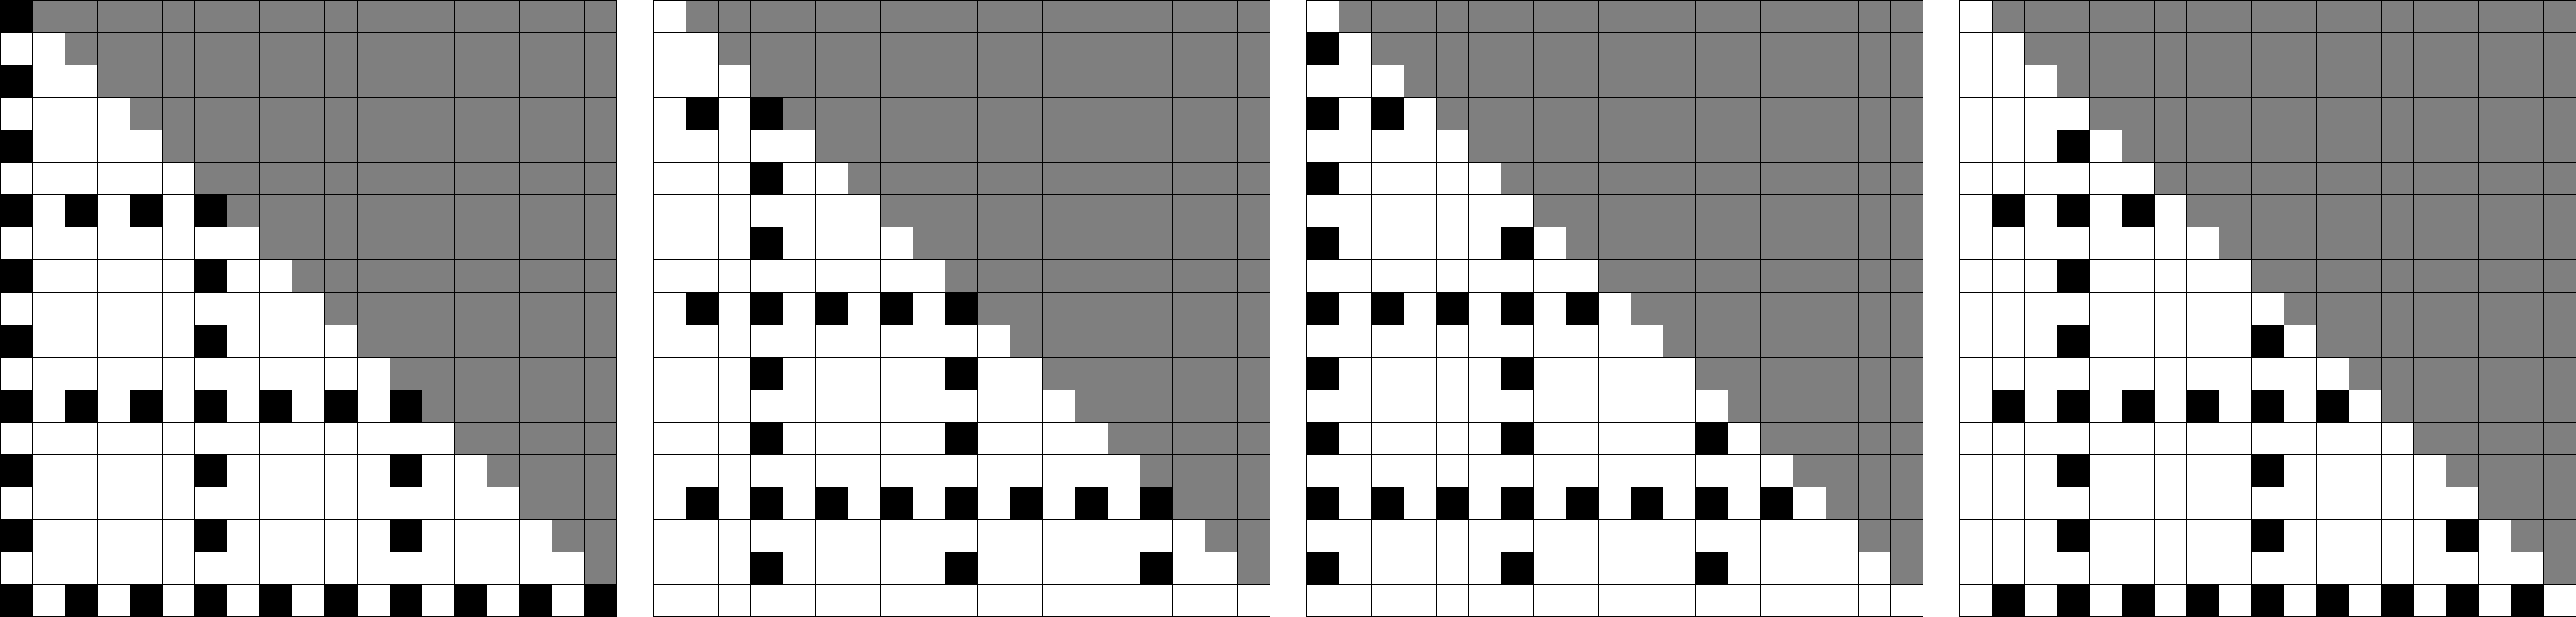
\includegraphics[width=\textwidth]{figures/4/thickness_6_case_1.pdf}
%\caption{Thickness 6 grids with perfect percolating sets as obtained in lemma \ref{lem:thickness_6_case_1} (left), and divisibility cases of thickness 6 (right).}
%\label{fig:thickness_6_case_1}
%\end{figure}

\begin{table}[]
\centering
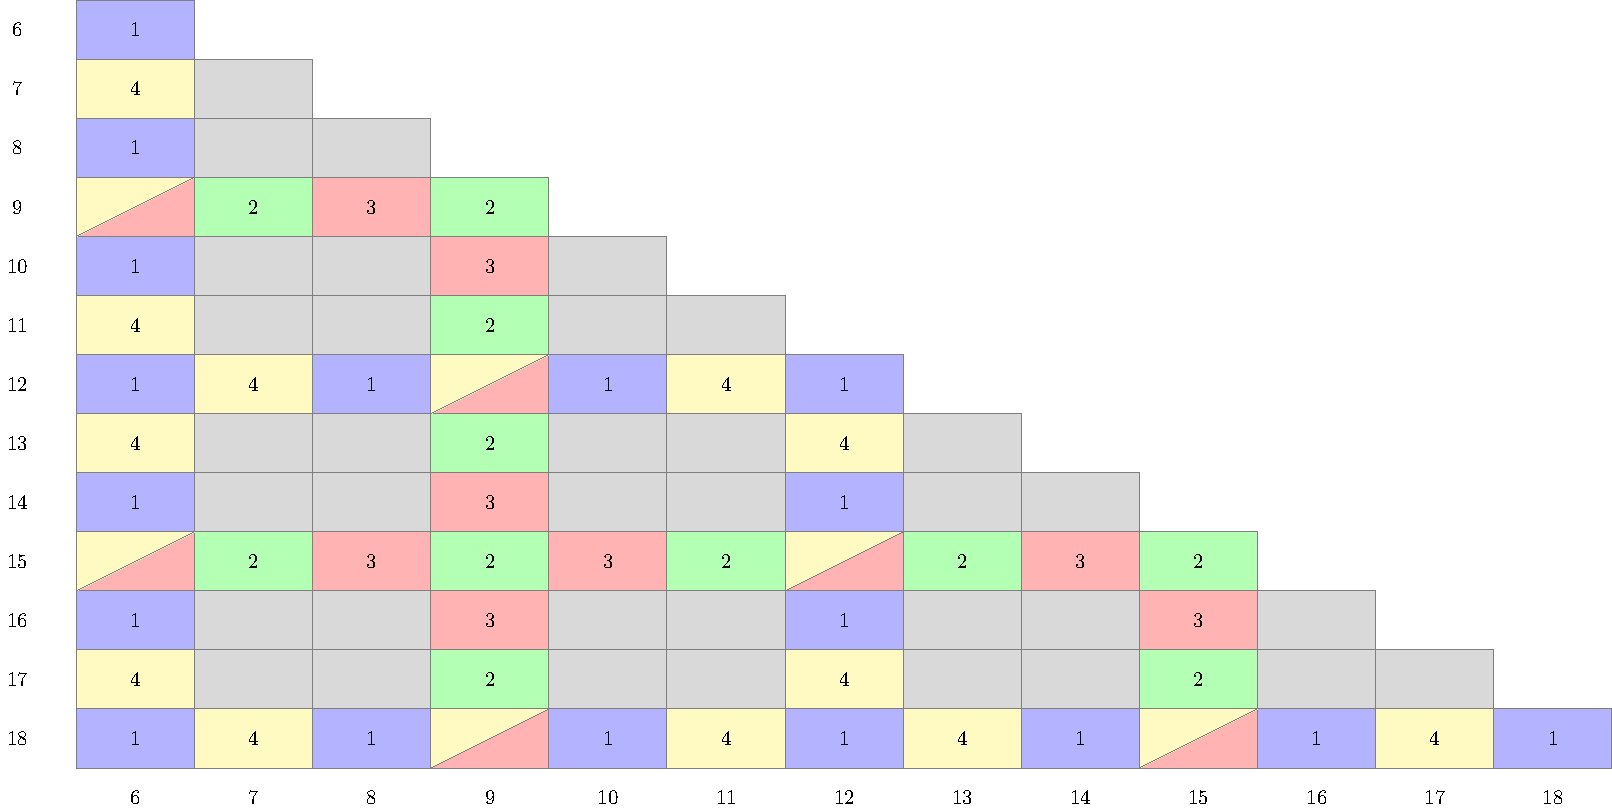
\includegraphics[width=\textwidth]{tables/4/thickness_6_cases.pdf}
\caption{The four thickness 6 cases analyzed in Lemmas \ref{lem:thickness_6_case_1} (blue), \ref{lem:thickness_6_case_2} (green), \ref{lem:thickness_6_case_3} (red), and \ref{lem:thickness_6_case_4} (yellow).}
\label{fig:thickness_6_cases}
\end{table}

\begin{lem}
\label{lem:thickness_6_case_1}
All grids $G(x,y,6)$ for $x \equiv 0 \pmod 6$, $y \equiv 0 \pmod 2$, and $x,y \geq 6$ admit perfect lethal sets.
\end{lem}

\begin{proof}
Consider $(3n,m,3) + (3,3,3)$, for $n,m \equiv 1 \pmod 2$ and $m > 1$. Observe that $(3n+3, m+3,6)$ obtains all grids of the form described in Case 1.

By Corollary \ref{cor:recursion}, we must show that $(3n,m,3), (3n,3,3), (3,m,3),(3,3,3)$ are all perfect. By Proposition \ref{prop:thickness_3_2d_family}, $(3n,m,3)$ is perfect for all $m > 1$. Since $n,m \neq 2$, $(3n,3,3), (3,m,3),(3,3,3)$ are all perfect by Proposition \ref{prop:3x3xk}. We conclude that all grids in Case 1 admit perfect lethal sets.
\end{proof}

\begin{lem}
\label{lem:thickness_6_case_2}
All grids $G(x,y,6)$ for $x \equiv 3 \pmod 6$, $y \equiv 1 \pmod 2$, and $x,y \geq 6$ admit perfect lethal sets.
\end{lem}

\begin{proof}
Consider $(3n,m,3) + (6,6,3)$, for $n,m \equiv 1 \pmod 2$ and $m > 1$. Observe that $(3n+6,m+6,6)$ obtains all grids of the form described in Case 2, apart from $G(x,7,6)$, for $x \equiv 3 \pmod 6$ and $x \geq 9$. 

By Corollary \ref{cor:recursion}, we must show that $(3n,m,3), (3n,6,3), (6,m,3), (6,6,3)$ are all perfect. By Proposition \ref{prop:thickness_3_2d_family}, $(3n,m,3)$ is perfect for all $m > 1$. Since $n,m > 1$, $(3n,6,3), (6,m,3), (6,6,3)$ are all perfect by Proposition \ref{prop:3x6xk}.

To obtain $(x,7,6)$, for $x \equiv 3 \pmod 6$ and $x \geq 9$, we consider $(6,3,3) + (x-6, 4,3)$. By Corollary \ref{cor:recursion}, we must show that $(6,3,3), (6,4,3), (x-6,3,3), (x-6,4,3)$ are all perfect. We obtain $(6,3,3)$ and $(x-6,3,3)$ from Proposition \ref{prop:3x6xk}. Proposition \ref{prop:3x6xk} gives $(6,4,3)$. Proposition \ref{prop:thickness_3_width_4} gives $(x-6,4,3)$. We conclude that all grids in Case 2 admit perfect lethal sets. 
\end{proof}

\begin{lem}
\label{lem:thickness_6_case_3}
All grids $G(x,y,6)$ for $x \equiv 3 \pmod 6$, $y \equiv 0 \pmod 2$, and $x,y \geq 6$ admit perfect lethal sets.
\end{lem}

\begin{proof}
Consider $(3n,m,3) + (6,3,3)$, for $n,m \equiv 1 \pmod 2$ and $m > 1$. Observe that $(3n+6,m+3,6)$ obtains all grids of the form described in Case 3. 

By Corollary \ref{cor:recursion}, we must show that $(3n,m,3), (3n,3,3), (6,m,3), (6,3,3)$ are all perfect. By Proposition \ref{prop:thickness_3_2d_family}, $(3n,m,3)$ is perfect for all $m > 1$. Since $m \neq 2$, $(6,m,3),(6,3,3)$ are both perfect by Proposition \ref{prop:3x3xk}. We obtain $(3n,3,3)$ by Proposition \ref{prop:3x3xk}. We conclude that all grids in Case 3 admit perfect lethal sets.
\end{proof}

\begin{lem}
\label{lem:thickness_6_case_4}
All grids $G(x,y,6)$, where $x \equiv 0 \pmod 6$, $y \equiv 1 \pmod 2$, and $x,y \geq 6$ admit perfect lethal sets.
\end{lem}

\begin{proof}
Consider $(3n,m,3) + (3,6,3)$, for $n,m \equiv 1 \pmod 2$ and $m > 1$. Observe that $(3n+3,m+6,6)$ obtains all grids described in Case 3, apart from $G(x,7,6)$, for $x \equiv 0 \pmod 6$ and $x \geq 6$. 

By Corollary \ref{cor:recursion}, we must show that $(3n,m,3)$, $(3n,6,3)$, $(3,m,3), (3,6,3)$ are all perfect. By Proposition \ref{prop:thickness_3_2d_family}, $(3n,m,3)$ is perfect for all $m > 1$. Since $n,m > 1$, $(3n,6,3)$ and $(3,6,3)$ are both perfect by Proposition \ref{prop:3x6xk}. Similarly, $(3,m,3)$ is perfect by Proposition \ref{prop:3x3xk}.

To obtain $(x,7,6)$, for $x \equiv 0 \pmod 6$ and $x \geq 6$, we consider $(3,3,3) + (x-3, 4,3)$. By Corollary \ref{cor:recursion}, we must show that $(3,3,3), (3,4,3), (x-3,3,3), (x-3,4,3)$ are all perfect. We obtain $(3,3,3), (3,4,3)$ and $(x-3,3,3)$ from Proposition \ref{prop:3x3xk}. Since $x \equiv 0 \pmod 6$, Proposition \ref{prop:thickness_3_width_4} gives $(x-3,4,3)$. We conclude that all grids given in Case 4 admit perfect lethal sets. 
\end{proof}

\begin{lem}
\label{lem:thickness_6_complete}
Thickness 6 is complete.
\end{lem}

\begin{proof}
All divisibility cases for thickness 6 are grids $G(x,y,6)$ such that at least one of $\{x,y\}$ is congruent to 0 modulo 3. Lemmas \ref{lem:thickness_6_case_1}, \ref{lem:thickness_6_case_2}, \ref{lem:thickness_6_case_3}, and \ref{lem:thickness_6_case_4} cover all such cases. The result follows.
\end{proof}

\section{Completeness of Thickness 7}

We show that all divisibility cases for grids of thickness 7 admit perfect lethal sets. Observe that divisibility cases for thickness 7 consist of grids $G(x,y,7)$ for $x,y$ in residue classes $\{0,1,3,4\}$ modulo 6 (see Table \ref{fig:thickness_7_cases}). We separate these divisibility cases into the following four cases and show that each case is complete:
\begin{enumerate}
\item $G(x,y,7)$ for $x,y \in \{1\} \pmod 3$, $x \equiv y \pmod 6$, and $x,y \geq 7$;
\item $G(x,y,7)$ for $x,y \in \{1\} \pmod 3$, $x \not\equiv y \pmod 6$, and $x,y \geq 7$;
\item $G(x,y,7)$ for $x,y \in \{0\} \pmod 3$, $x \equiv y \pmod 6$, and $x,y \geq 7$;
\item $G(x,y,7)$ for $x,y \in \{0\} \pmod 3$, $x \not\equiv y \pmod 6$, and $x,y \geq 7$.
\end{enumerate}

\begin{table}[]
\centering
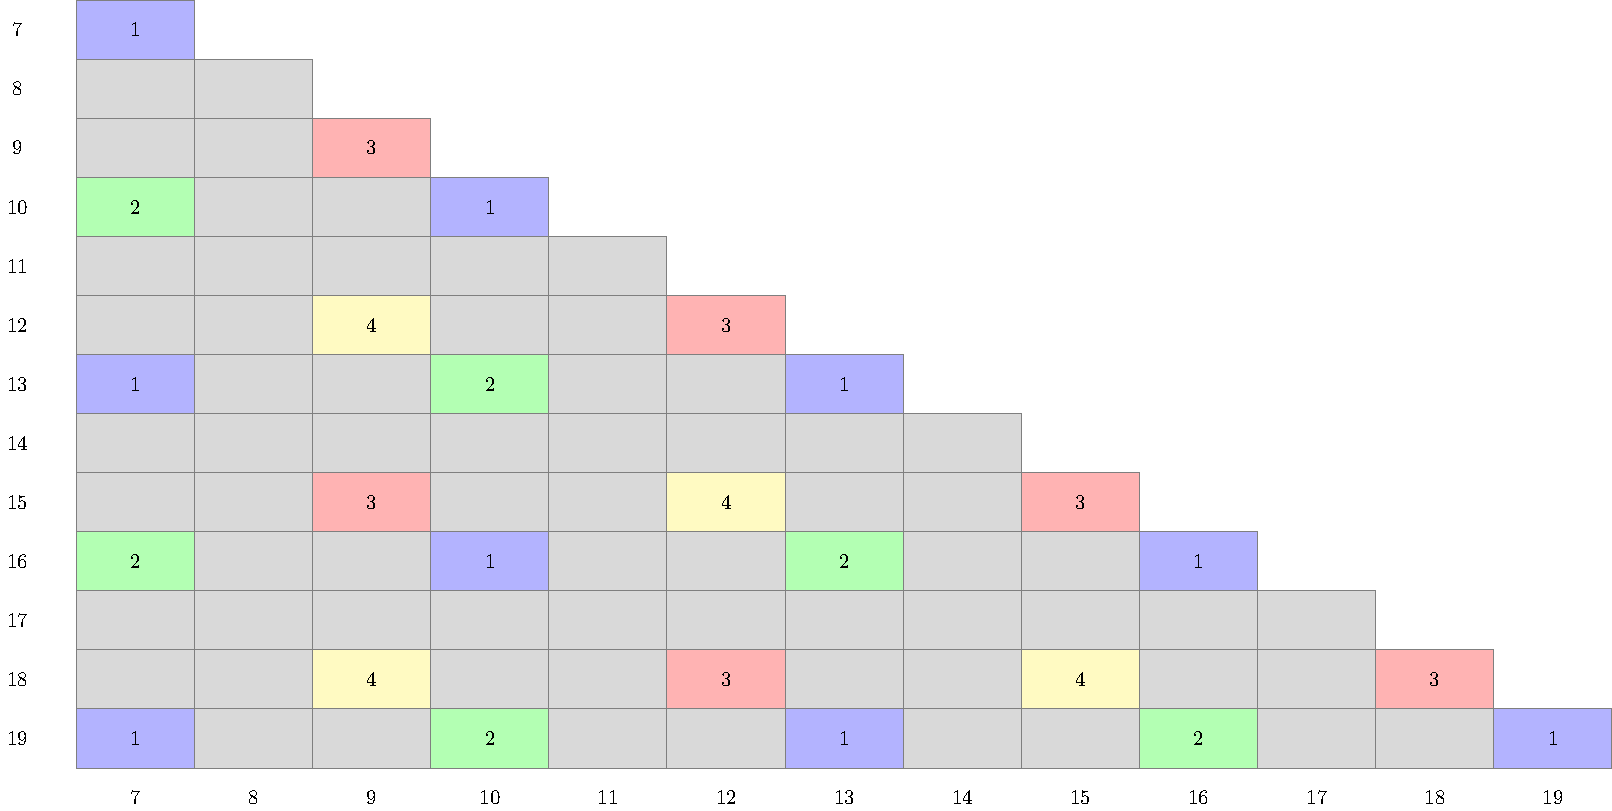
\includegraphics[width=\textwidth]{tables/4/thickness_7_cases.pdf}
\caption{The four thickness 7 cases analyzed in Lemmas \ref{lem:thickness_7_case_1} (blue), \ref{lem:thickness_7_case_2} (green), \ref{lem:thickness_7_case_3} (red), and \ref{lem:thickness_7_case_4} (yellow).}
\label{fig:thickness_7_cases}
\end{table}

\begin{lem}
\label{lem:thickness_7_case_1}
All grids $G(x,y,7)$ for $x,y \in \{1,4\}$, $x \equiv y \pmod 6$, and $x,y \geq 7$ admit perfect lethal sets.
\end{lem}

\begin{proof}
Consider $(a,b,2) + (8,5,5)$ for $a,b \in \{2,5\} \pmod 6$, $a \not\equiv b \pmod 6$, and $a,b > 2$. Observe that $(a+8,b+5,7)$ obtains all grids described in Case 1 above, apart from $G(10,10,7)$ and $G(a, 7,7)$, for $a \equiv 1 \pmod 6$. 

By Corollary \ref{cor:recursion}, we must show that $(a,b,2), (a,5,5), (8,b,5), (8,5,2)$ are all perfect. By Proposition \ref{prop:thickness_2_2d_family}, $(a,b,2)$ and $(8,5,2)$ are perfect. By Lemma \ref{lem:thickness_5_complete}, $(a,5,5)$ and $(8,b,5)$ are perfect. 

To obtain $(a,7,7)$, for $a \equiv 1 \pmod 6$ and $a \ge 7$, we consider $(4,4,4) + (a-4,3,3)$. By Corollary \ref{cor:recursion}, we must show that $(4,4,4), (4,3,3), (a-4,4,3), (a-4,3,4)$ are all perfect. By Theorem \ref{thm:hypercubes}, we have that $(2,2,2)$ and $(4,4,4)$ are perfect. Proposition \ref{prop:3x3xk} gives $(4,3,3)$. Since $a-4 \equiv 3 \pmod 6$, we obtain $(a-4,4,3)$ from Proposition \ref{prop:thickness_3_width_4}.

To obtain $(10,10,7)$, consider $(5,5,5) + (5,5,2)$. By Corollary \ref{cor:recursion}, we must show that $(5,5,5), (5,5,2), (5,5,2), (5,5,5)$ are all perfect. Lemma \ref{lem:thickness_5_complete} gives us $(5,5,5)$, and Construction \ref{con:5x5x2} gives us $(5,5,2)$. We conclude that all grids in Case 1 admit perfect lethal sets. 
\end{proof}

\begin{lem}
\label{lem:thickness_7_case_2}
All grids $G(x,y,7)$ for $x,y \in \{1,4\}$, $x \not\equiv y \pmod 6$, and $x,y \geq 7$ are complete.
\end{lem}

\begin{proof}
Consider $(a,b,2) + (5,5,5)$ for $a,b \in \{2,5\} \pmod 6$, $a \not\equiv b \pmod 6$, and $a,b > 2$. Observe that $(a+5,b+5,7)$ obtains all grids described in Case 2 above, apart from $G(a,7,7)$, for $a \equiv 4 \pmod 6$. 

By Corollary \ref{cor:recursion}, we must show that $(a,b,2), (a,5,5), (5,b,5), (5,5,2)$ are all perfect. By Proposition \ref{prop:thickness_2_2d_family}, $(a,b,2)$ is perfect. We obtain $(a,5,5)$ and $(5,b,5)$ from Lemma \ref{lem:thickness_5_complete}, and $(5,5,2)$ is given by Construction \ref{con:5x5x2}.

To obtain $(a,7,7)$, for $a \equiv 4 \pmod 6$, we consider $(7,4,4) + (a-7,3,3)$. Since $a \equiv 4 \pmod 6$ and $a \geq 7$, we have that $a \geq 10$. By Corollary \ref{cor:recursion}, we must show that $(7,4,4), (7,3,3), (a-7,4,3), (a-7,3,4)$ are all perfect. We obtain $(7,4,4)$ from $(2,2,2) + (5,2,2)$. Theorem \ref{thm:hypercubes} and Construction \ref{con:5x2x2} show that $(2,2,2)$, $(2,2,2)$, $(5,2,2)$, $(5,2,2)$ are all perfect. Proposition \ref{prop:3x3xk} gives us $(7,3,3)$. Since $a-7 \equiv 3 \pmod 6$, we obtain $(a-7,4,3)$ from Proposition \ref{prop:thickness_3_width_4}. We conclude that all grids in Case 2 admit perfect lethal sets. 
\end{proof}

\begin{lem}
\label{lem:thickness_7_case_3}
All grids $G(x,y,7)$ for $x,y \in \{0,3\}$, $x \equiv y \pmod 6$, and $x,y \geq 7$ are complete.
\end{lem}

\begin{proof}
Consider $(a,b,2) + (6,9,5)$ for $a,b \in \{0,3\} \pmod 6$, $a \not\equiv b \pmod 6$, and $a,b > 2$. Observe that $(a+6,b+9,7)$ contains all grids described in Case 3 above, apart from $G(9,9,7)$. 

By Corollary \ref{cor:recursion}, we must show that $(a,b,2), (a,9,5), (6,b,5), (6,9,2)$ are all perfect. By Proposition \ref{prop:thickness_2_2d_family}, $(a,b,2)$ and $(6,9,2)$ are perfect. By Proposition \ref{prop:thickness_3_2d_family}, $(a,9,5)$ is perfect. We obtain $(6,b,5)$ from Lemma \ref{lem:thickness_5_complete}, for $b \geq 5$, and $(6,3,5)$ from Proposition \ref{prop:3x6xk}. 

To obtain $(9,9,7)$, consider $(6,6,4) + (3,3,3)$. By Corollary \ref{cor:recursion}, we must show that $(6,6,4), (6,3,3), (3,6,3), (3,3,4)$ are all perfect. We obtain $(6,6,4)$ from $(3,3,1) + (3,3,3)$. Construction \ref{con:3x3x1} shows that $(3,3,1)$ is perfect. Proposition \ref{prop:3x3xk} gives us $(6,3,3)$, $(3,3,3)$ and $(4,3,3)$. We conclude that all grids in Case 3 admit perfect lethal sets.
\end{proof}

\begin{lem}
\label{lem:thickness_7_case_4}
All grids $G(x,y,7)$ for $x,y \in \{0,3\}$, $x \not\equiv y \pmod 6$, and $x,y \geq 7$ are complete.
\end{lem}

\begin{proof}
Consider $(a,b,2) + (6,6,5)$ for $a,b \in \{0,3\} \pmod 6$, $a \not\equiv b \pmod 6$, and $a,b > 2$. Observe that $(a+6,b+6,7)$ contains all grids described in Case 4 above. 

By Corollary \ref{cor:recursion}, we must show that $(a,b,2), (a,6,5), (6,b,5), (6,6,2)$ are all perfect. By Proposition \ref{prop:thickness_2_2d_family}, $(a,b,2)$ is perfect. We obtain $(6,b,5)$ from Lemma \ref{lem:thickness_5_complete}, for $b \geq 5$, and $(6,3,5)$ from Proposition \ref{prop:3x6xk}. We obtain $(6,6,2)$ from $(3,3,1)+(3,3,1)$. By Proposition \ref{prop:purina}, $(3,3,1)$ is perfect, and so by Corollary \ref{cor:recursion}, $(6,6,2)$ is perfect. We conclude that all grids in Case 4 admit perfect lethal sets.
\end{proof}

\begin{lem}
Thickness 7 is complete.
\end{lem}

\begin{proof}
\label{lem:thickness_7_complete}
By Lemmas \ref{lem:thickness_7_case_1}, \ref{lem:thickness_7_case_2}, \ref{lem:thickness_7_case_3}, and \ref{lem:thickness_7_case_4}, all divisibility cases for thickness 7 admit perfect lethal sets.
\end{proof}

\section{Proof of the Main Result}

We are now in a position to prove Theorem \ref{thm:main_result}. We first state the following auxiliary result for divisibility cases. 

\begin{cor}
\label{cor:divisibility_complete}
Let $G(a_1,a_2,a_3)$ be a divisibility case, for $a_1, a_2, a_3 \geq 5$. Then $(a_1,a_2,a_3)$ is perfect.
\end{cor}

\begin{proof}
By Lemmas \ref{lem:thickness_5_complete}, \ref{lem:thickness_6_complete}, and \ref{lem:thickness_7_complete}, all divisibility cases for $G(a_1,a_2,5)$, $G(a_1,a_2,6)$, and $G(a_1,a_2,7)$ admit perfect lethal sets. Observe that $(a_1,a_2,a_3) + (3,3,3)$ gives a one-to-one mapping from divisible grids of thickness $a_3$ to divisible grids of thickness $a_3+3$. By Lemma \ref{lem:plus_333}, if $(a_1,a_2,a_3)$ is perfect, then $(a_1,a_2,a_3) + (3,3,3)$ is perfect. Therefore, since each residue class modulo 3 is complete, all divisibility cases $G(a_1,a_2,a_3)$, for $a_1, a_2, a_3 \geq 5$, admit perfect lethal sets.
\end{proof}

The proof of Theorem \ref{thm:main_result} requires further implementation of the recursive process outlined in Lemma \ref{lem:recursion}. In particular, we leverage Corollary \ref{cor:divisibility_complete} to prove the following helpful lemma:

%\begin{lem}
%Let $(a_1,a_2,a_3)$ be any grid such that $a_1 \geq a_2 \geq a_3 \geq 5$. Let $b_1, b_2, b_3$ be integers such that $b_1 \equiv b_2 \equiv b_3 \equiv 0 \pmod 3$ and $b_1, b_2, b_3 \geq 6$. Suppose $(a_1,a_2,a_3)$ admits an optimal lethal set. Then $(a_1,a_2,a_3) + (b_1,b_2,b_3)$ is optimal.
%\end{lem}

%\begin{proof}
%By Corollary \ref{cor:recursion}, we must show that $(a_1,b_2,b_3), (b_1,a_2,b_3), (b_1,b_2,a_3)$ are all perfect. Since $b_1 \equiv b_2 \equiv b_3 \equiv 0 \pmod 3$, each of these grids is divisible. Furthermore, since $a_1,a_2,a_3,b_1, b_2, b_3 \geq 5$, by Corollary \ref{cor:divisibility_complete}, each grid is perfect.
%\end{proof}

\begin{lem}
\label{lem:multiples_of_3}
Let $G(a_1,a_2,a_3)$ be any grid such that $a_1, a_2, a_3 \geq 5$. If $(a_1,a_2,a_3)$ is optimal, then $(a_1,a_2,a_3) + (3b_1,3b_2,3b_3)$ is optimal for $b_1,b_2,b_3 \geq 2$. 
\end{lem}

\begin{proof}
By Corollary \ref{cor:recursion}, we must show that $(a_1,3b_2,3b_3), (3b_1,a_2,3b_3), (3b_1,3b_2,a_3)$ are all perfect. Since $3b_1 \equiv 3b_2 \equiv 3b_3 \equiv 0 \pmod 3$, each of these grids is divisible. Furthermore, each grid has minimum thickness 5 and so, by Corollary \ref{cor:divisibility_complete}, each grid is perfect.
\end{proof}

Let $(r_1,r_2,r_3)$ be the tuple of residues of $(a_1,a_2,a_3)$ modulo 3. Given an optimal grid $G(a_1,a_2,a_3)$ such that $a_1,a_2,a_3 \ge 5$, Lemma \ref{lem:multiples_of_3} says that all other grids of size at least $G(a_1+6,a_2+6,a_3+6)$ with the same $(r_1,r_2,r_3)$ are optimal. Therefore, by obtaining optimal lethal sets on the smallest grids for each residue tuple $(r_1,r_2,r_3)$, we are able to obtain a lower bound on the size of all optimal grids under 3-neighbor percolation (see Table \ref{tab:residues}).

\begin{table}[]
\centering
\begin{subfigure}{0.3\textwidth}
	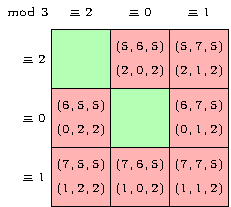
\includegraphics[width=\textwidth]{tables/4/residue_2.pdf}
	%\caption{Thickness 5}
	\label{tab:r_a}
\end{subfigure} \hfill%
\begin{subfigure}{0.3\textwidth}
	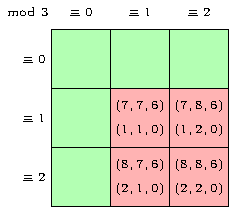
\includegraphics[width=\textwidth]{tables/4/residue_0.pdf}
	%\caption{Thickness 6}
	\label{tab:r_b}
\end{subfigure} \hfill%
\begin{subfigure}{0.3\textwidth}
	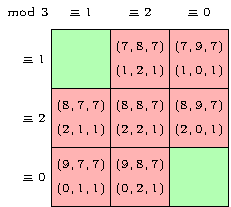
\includegraphics[width=\textwidth]{tables/4/residue_1.pdf}
	%\caption{Thickness 7}
	\label{tab:r_c}
\end{subfigure}
\caption{Residue tuples for non-divisibility cases in thicknesses 5, 6, and 7. Top tuple is grid dimension, bottom tuple is residues modulo 3.}
\label{tab:residues}
\end{table} 

\begin{proof}[Proof of Theorem \ref{thm:main_result}]
Let $(a_1,a_2,a_3)$ be such that $a_1, a_2, a_3 \geq 11$. Observe that each $a_i$ can be written as $3b_i + r_i$, for $b_i \geq 2$ and some $r_i \in \{5,6,7\}$. We therefore have that $(a_1,a_2,a_3) = (r_1,r_2,r_3) + (3b_1,3b_2,3b_3)$, for $r_1,r_2,r_3 \in \{5,6,7\}$. By Lemma \ref{lem:multiples_of_3}, $(a_1,a_2,a_3)$ is optimal if $(r_1,r_2,r_3)$ is optimal. 

Corollary \ref{cor:divisibility_complete} gives us the optimality of divisibility cases. Therefore, we need only consider non-divisible grids $G(r_1,r_2,r_3)$. In particular, we must show that $(6,5,5)$, $(7,5,5)$, $(7,6,5)$, $(7,7,5)$ and $(7,7,6)$ are all optimal. We obtain $(7,7,6)$ from $(4,4,3) + (3,3,3)$. The construction for $(4,4,3)$ is given in Construction \ref{con:4x4x3}. By Lemma \ref{lem:plus_333}, $(7,7,6)$ is optimal. Constructions for $(6,5,5)$, $(7,5,5)$, $(7,6,5)$, $(7,7,5)$ are given in Appendix A.

Since each of the non-divisibility grids $G(r_1,r_2,r_3)$ admits an optimal lethal set, we conclude that all grids $G(a_1,a_2,a_3)$ where $a_1, a_2, a_3 \geq 11$ are optimal.
\end{proof}

%\begin{lem}
%Let $R$ be a minimum set of grids representing each unique non-divisible residue tuple modulo 3. Without loss of generality, suppose $a_1 \geq a_2 \geq a_3$ for all $(a_1,a_2,a_3) \in R$, and let $a$ be the minimum value of $a_3$. If each $G \in R$ admits an optimal lethal set, then all non-divisible grids $(a_1,a_2,a_3)$, where $a_1, a_2, a_3 \geq a+6$, are optimal.
%\end{lem}

% COMMENT
% COMMENT
% COMMENT
% COMMENT
% COMMENT

\begin{comment}

Let $(a,b,2)$ represent an arbitrary (divisible) grid of thickness 2, and let $x = a \pmod 6$ and $y = b \pmod 6$. By \{some as of yet unwritten construction\}, we have that $(a,b,2)$ percolates at the lower bound for all $x,y \in \{0,2,3,5\}$, where $x \neq y$. We consider two constructions: $(a,b,2) + (6,3,3)$ and $(a,b,2) + (6,6,3)$. 

By item (1) of the remark, in order to show that $(a,b,2) + (6,3,3)$ percolates at the lower bound, it is sufficient to show that $(a,b,2), (a,3,3), (6,b,3), (6,3,2)$ all percolate at the bound. By \{more unwritten constructions\}, this is true for all $x,y \in \{0,2,3,5\}$, where $x \neq y$, $a,b > 1$, and at least one of $\{a,b\} > 2$. (Note that if $a=2$, one of the tuples is $(2,3,3)$, which does not percolate at the lower bound; we accommodate for this by re-writing $(a,b,2) + (6,3,3)$ as $(a,b,2) + (3,6,3)$.) The resulting tuple $(a', b', 5)$ is a grid of thickness 5, with $a'$ and $b'$ in the same residue class modulo $6$, $x,y \geq 8$, and at least one of $\{a',b'\} \geq 9$. From \{some figure representing the divisibility cases of thickness 5\}, we see that the lower bound on $a'$ and $b'$ omits all grids of the form $(5,5,k)$ and $(5,6,k)$, as well as the singular grid $(8,8,5)$. 

Applying an analogous argument to $(a,b,2) + (6,6,3)$, we must demonstrate that $(a,b,2), (a,6,3), (6,b,3), (6,6,2)$ all percolate at the lower bound. By \{some other constructions\}, we again find that this holds for all $x,y \in \{0,2,3,5\}$, where $x \neq y$ and $a,b > 1$. This gives all thickness 5 tuples $(a',b', 5)$ with $a'$ and $b'$ in different residue classes modulo $6$, where $a',b' \geq 8$. 

Combining these results, we have completeness for all grids of thickness 5 except those of the form $(5,5,k)$ and $(5,6,k)$, and the singular grid $(8,8,5)$. By lemmas \ref{lem:width_5} and \ref{lem:width_6}, and \{some construction for $(8,8,5)$\}, these cases are also complete, and so thickness 5 is complete. This completes the proof. 

\end{comment}




